\documentclass[12pt]{article}

\usepackage{lineno,amsmath,listings,textcomp,needspace,graphicx,gensymb}
\usepackage{xcolor}
\usepackage[hidelinks]{hyperref}
\usepackage{graphicx}
\usepackage{caption}
\usepackage{subcaption}

\definecolor{backcolour}{rgb}{0.95,0.95,0.92}

\lstdefinestyle{code_blocks}{
    backgroundcolor=\color{backcolour},  
    basicstyle={\linespread{0.8}\small\ttfamily},
    breakatwhitespace=false,         
    breaklines=true,                 
    captionpos=b,                    
    keepspaces=true,                 
    numbers=left,                    
    numbersep=5pt,                  
    showspaces=false,                
    showstringspaces=false,
    showtabs=false,                  
    tabsize=2
}
\lstset{style=code_blocks}


\title{Sample Figures}
\author{Patrick Johnson}
\date{\today}

\begin{document}
\maketitle
\newpage

Examples of figures. Figure~\ref{fig:fig_1}, Figure~\ref{fig:multi_1}, and Figure~\ref{fig:multi_2}

\begin{figure}
    \centering
    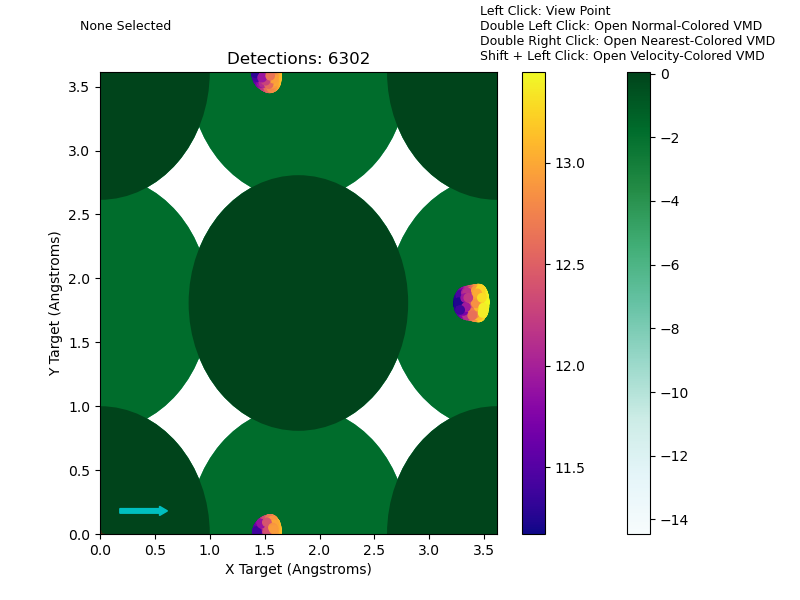
\includegraphics[width=0.98\textwidth]{fig_1.png}
    \caption{Sample Figure.}
    \label{fig:fig_1}
\end{figure}

\begin{figure}[ht]
    \begin{subfigure}{.495\textwidth}
      \centering
      % include first image
      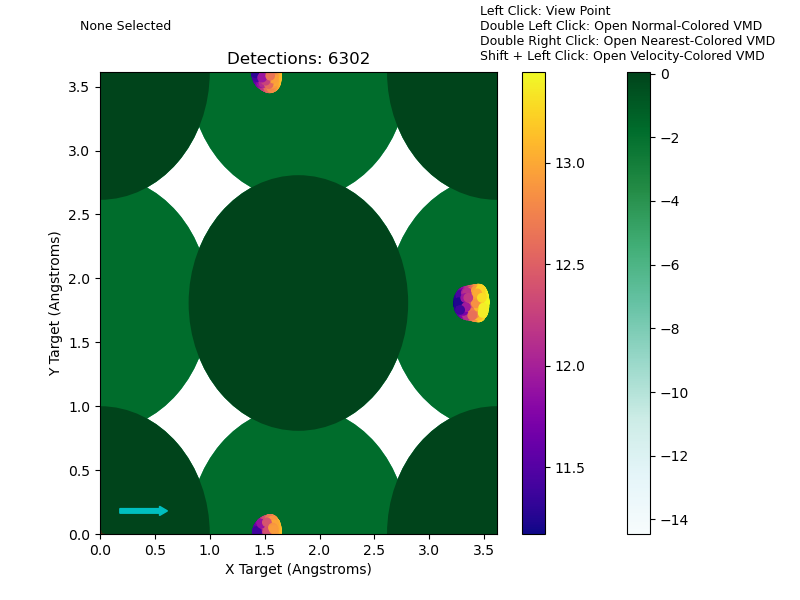
\includegraphics[width=1\linewidth]{fig_1.png}  
      \caption{Test a}
      \label{fig:multi_1_a}
    \end{subfigure}
    \begin{subfigure}{.495\textwidth}
      \centering
      % include second image
      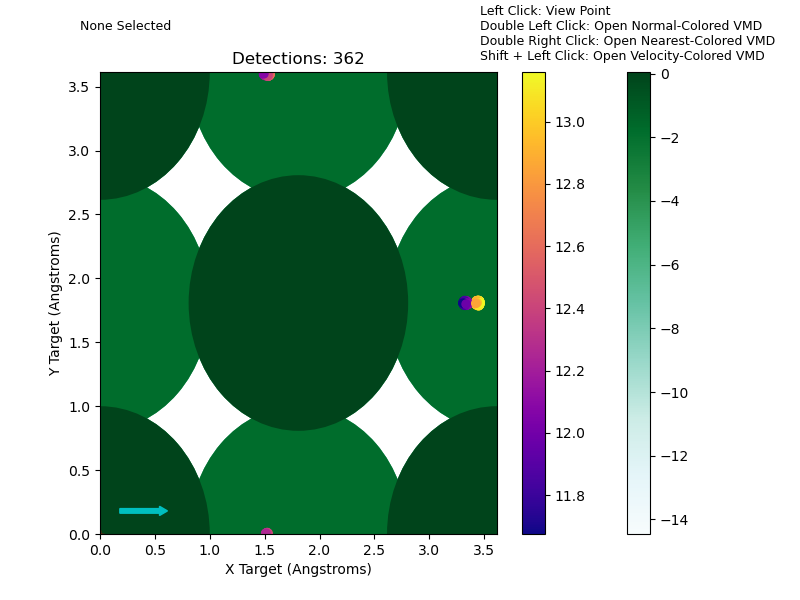
\includegraphics[width=1\linewidth]{fig_2.png}  
      \caption{Test b}
      \label{fig:multi_1_b}
    \end{subfigure}
    \caption{Sample Multi Horizontal Figure. (\ref{sub@fig:multi_1_a}) - (\ref{sub@fig:multi_1_b}), Figure~\ref{fig:multi_1_a}, Figure~\ref{fig:multi_1_b}}
    \label{fig:multi_1}
\end{figure}

\begin{figure}[ht]
    \begin{subfigure}{.95\textwidth}
      \centering
      % include first image
      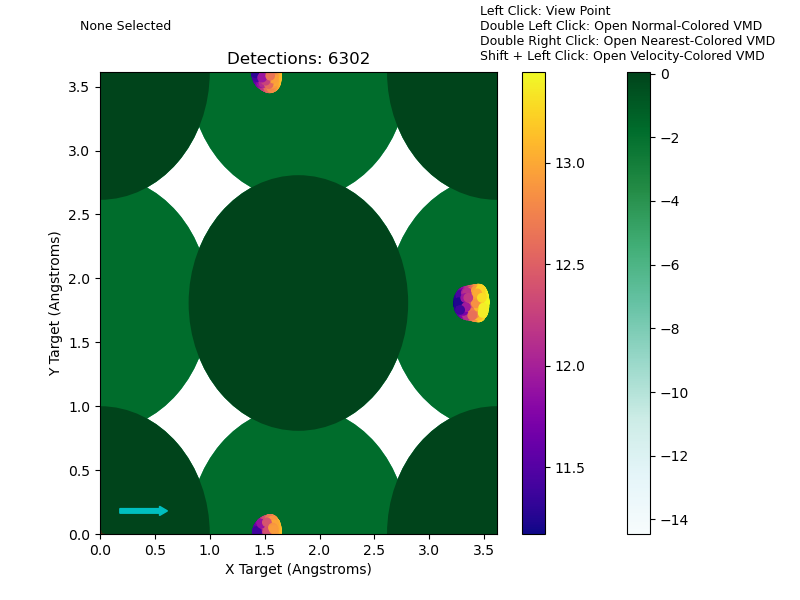
\includegraphics[width=1\linewidth]{fig_1.png}  
      \caption{Test a}
      \label{fig:multi_2_a}
    \end{subfigure}
    \newline
    \begin{subfigure}{.95\textwidth}
      \centering
      % include second image
      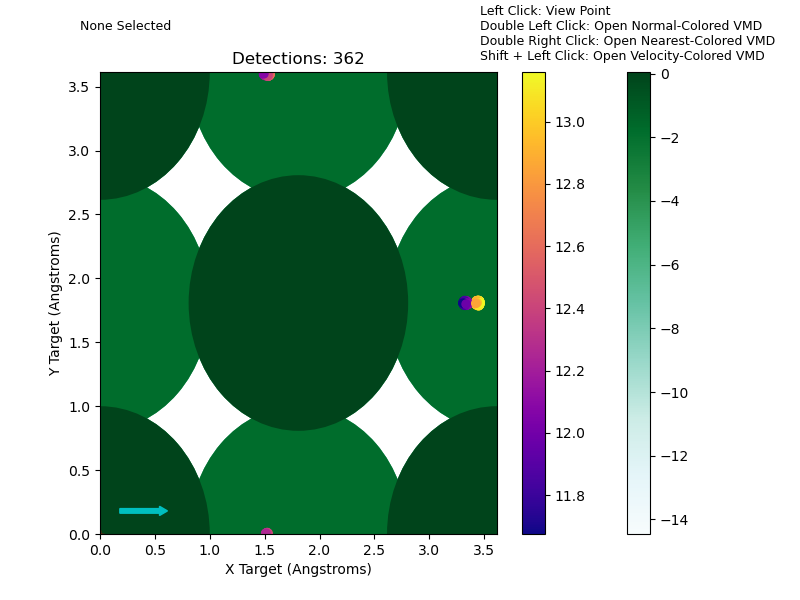
\includegraphics[width=1\linewidth]{fig_2.png}  
      \caption{Test b}
      \label{fig:multi_2_b}
    \end{subfigure}
    \caption{Sample Multi Vertical Figure. (\ref{sub@fig:multi_2_a}) - (\ref{sub@fig:multi_2_b})), Figure~\ref{fig:multi_2_a}, Figure~\ref{fig:multi_2_b}}
    \label{fig:multi_2}
\end{figure}


\end{document}